\newcommand{\mypathoj}{../thesis/oj}

\newcommand{\mypathojdata}{../thesis/oj/data}
\newcommand{\alert}[1]{#1}
\chapter{Reducing~Cascading~Risk~Through  Real-Time~Dispatch}\label{ch:jccow}

Large scale load shedding events caused by cascading power failures have an extreme impact on society.  As seen in \Cref{intro-chapter}, the costs of these single events can be in the billions, put a halt on commercial and industrial activities, and even cause the loss of life.  In this Chapter, we extend our joint chance-constrained model to more effectively control line failures that may lead to large load-shedding events.


The downside of a chance constrained model is that it does not account for the impact of failure events.  Power system networks are comprised of many different classes of assets.  The most straightforward example is that the failure of a small distribution line in a radial tree has minimal impact on the reliability of the bulk power system and the high voltage network that carries the majority of the power over long distances.  However, even among the bulk power system, the failure of individual lines may have disproportionate impact on the probability of a large scale cascading event.  This may have to do with many things such as the connectivity of a neighboring node, the current environmental conditions in and around a region, or even the relay settings on neighboring transmission lines.  Here we take an empirical approach using the OPA cascading simulation from \Cref{dfo-chapter} to evaluate the impact of losing a line on the resulting cascade simulation and the output of the load shed distribution.  We then incorporate this measure of impact into our JCC model by giving it an OPA weighting scheme, denoted JCC-OW (Joint Chance Constraint - OPA Weighted).  This OPA weighting scheme can be thought of as a surrogate model for OPA to be used in a real time dispatch model.  This problem is solved with a cutting plane algorithm similar to JCC.  Finally, we explore the trade-off between cost of dispatch and rare event risk through the computational section.




\section{Cascading Failure Risk Model}
We would like to take into account the impact of losing a transmission element on the load shed distribution from OPA.  Instead of being concerned with only whether or not a line fails, we would also like to know how much does this line contribute to cascading power failure risk.  Due to reliability requirements such as $N-1$ constraints, the base system is typically stable and has low cascading power failure risk.  Since line failures can be caused by things outside of system control, we perform our risk analysis under $N-1$ exogenous contingencies corresponding to each individual line failure.  After these initial line failures the system is sometimes moved to a state where additional failures may begin a cascading process leading to a large load shed event.  We use these $N-1$ contingencies as well as our JCC risk model to sample initial contingencies for the OPA cascading process.  The initial contingency includes the line that failed with certainty due to an exogenous event as well as probable line failures due to current flow on transmission elements.  We use the distribution of load shed after the OPA process to develop a weighting for the  JCC model to take into account the effects of the particular line on the cascading process. 

\subsection{Overview of Sources of Uncertainty}

\begin{figure}
\centering
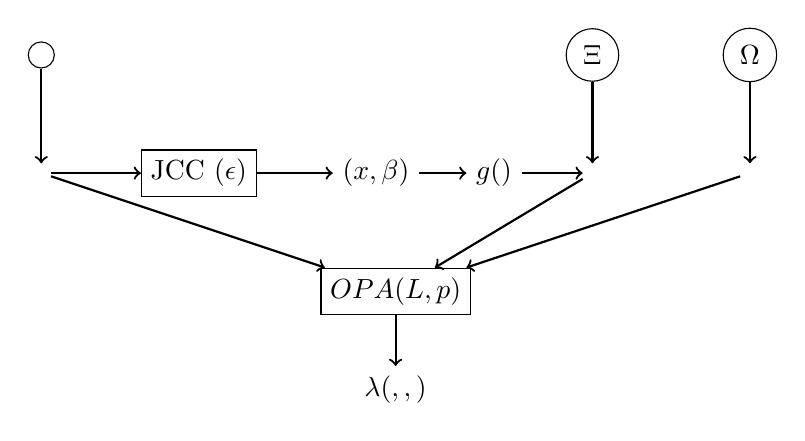
\begin{tikzpicture}

\draw (0,3.5) node(demand)[circle,draw]{ $\bD$};
\draw (7,3.5) node(contingency)[circle,draw]{ $\Xi$};
\draw (9,3.5) node(evolution)[circle,draw]{ $\Omega$};

\draw (0,2) node(rd){ $\rd $};
\draw (2,2) node(JCC)[rectangle,draw]{ JCC $(\epsilon)$ };
\draw (4.25,2) node(rf){ $\ry(x,\beta)$};
\draw (5.75,2) node(grf){ $g(\ry)$};
\draw (7,2) node(rxi){ $\rxi$};
\draw (9,2) node(romega){ $\romega$};
\draw (4.5,.5) node(ropa)[rectangle,draw]{ $OPA(L,p)$};
\draw (4.5,-.75) node(rlambda){ $\lambda(\rd,\rxi,\romega)$};

\draw[thick,->] (demand) -- (rd);
\draw[thick,->] (rd) -- (JCC);
\draw[thick,->] (JCC) -- (rf);
\draw[thick,->] (rf) -- (grf);
\draw[thick,->] (grf) -- (rxi);
\draw[thick,->] (contingency) -- (rxi);
\draw[thick,->] (evolution) -- (romega);
\draw[thick,->] (rd) -- (ropa);
\draw[thick,->] (rxi) -- (ropa);
\draw[thick,->] (romega) -- (ropa);
\draw[thick,->] (ropa) -- (rlambda);

\end{tikzpicture} 
\caption{Random variable relationships and sources of uncertainty}\label{randomrelationship}
\end{figure}

We are capturing three separate sources of uncertainty and evaluating the stress on the power system by using the OPA cascading model as a surrogate process for the risk of a cascading power failure.  The power system is affected by the uncertainty in demand and generation, denoted by random variable $\rd = d + C_m \ri$ with  probability space associated with $\bD$.  We built this uncertainty into our model by assuming the net injection uncertainty is multivariate Gaussian, we calculate a system risk measure approximating the probability that one or more lines fail.  This ties into the next source of uncertainty, encapsulated by the  random variable $\rxi$ for probability space $\Xi$, which models the initial line failures that could initiate a cascading sequence.  This random variable, $\rxi$, provides the connection between the JCC model of \Cref{jcc-chapter} with the OPA model from \Cref{msip-model,dfo-chapter}.  The primary source of uncertainty modeled in \Cref{msip-model,dfo-chapter} was encapsulated in the random variable  $\romega$ from a sample space $\Omega$ which governs the evolution of the cascading model.  This cascading model can be seen as a surrogate for the stress on the power system in relation to rare event failures.     

The JCC model incorporates uncertainty from random demand, $\ri$.  The outcome of the JCC model are random variables for branch flows.  Using a failure density function from the probability space associated with $\Xi$, we find a distribution of initial contingencies $\xi$.  The OPA model incorporates uncertainty from all three sources, the demand $\bD$, the initial contingencies $\Xi$, and the cascade evolution $\Omega$.  Let $\cX = \bD \times \Xi \times \Omega$ represent the whole sample space underlying the probability space for the OPA model, where $\rchi = (\rd, \rxi, \romega)$ is an event in the larger sample space.  The random variables' dependencies are laid out in \Cref{randomrelationship} that describe the relationships between variables.



\subsection{$N-1$ Exogenous Contingencies}

\begin{figure}
\centering
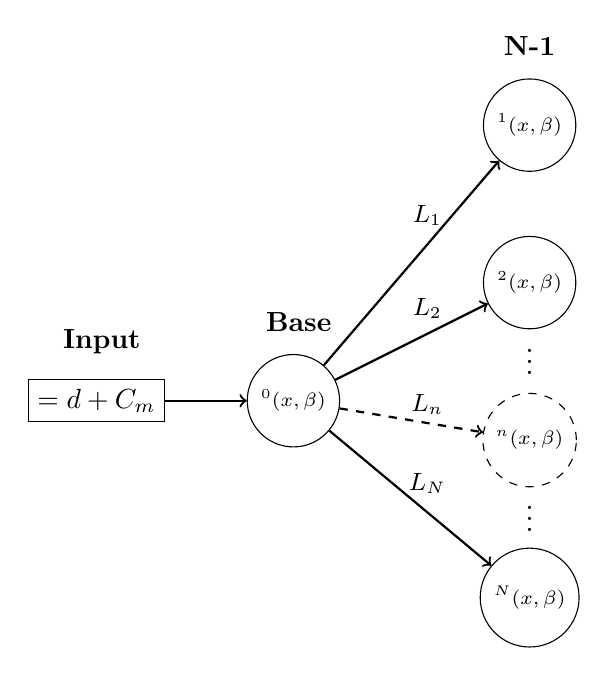
\begin{tikzpicture}

\draw (-2,1.25) node{ \textbf{ Input} };
\draw (-2,.5) node(INPUT)[rectangle,draw]{ $\rd=d + C_m \rdelm$};
\draw (.5,1.5) node{ \textbf{ Base} };
\draw (.5,.5) node(ROOT)[circle,draw]{\scriptsize $\ry^0(x,\beta)$ };
\draw (3.5,5) node{ $\textbf{N-1}$ };
\draw (3.5,4) node(ONE)[circle,draw]{ \scriptsize $\ry^1(x,\beta)$ };
\draw (3.5,2) node(TWO)[circle,draw]{ \scriptsize $\ry^2(x,\beta)$ };
\draw (3.5,1.1) node(DOTONE){ \large $\vdots$ };
\draw (3.5,0) node(N)[circle,dashed,draw]{ \scriptsize $\ry^n(x,\beta)$ };
\draw (3.5,-.9) node(DOTTWO){ \large $\vdots$ };
\draw (3.5,-2) node(S)[circle,draw]{ \scriptsize $\ry^N(x,\beta)$ };

\draw (2.2,2.85) node(OMG1){ \small $L_1$ };
\draw (2.2,1.67) node(OMG2){ \small $L_2$ };
\draw (2.2,.45) node(OMG){ \small $L_n$ };
\draw (2.2,-.55) node(OMGS){ \small $L_N$ };


\draw[thick, ->] (INPUT) -- (ROOT) ;
\draw[thick, ->] (ROOT) -- (ONE) ;
\draw[thick,->] (ROOT) -- (TWO);
\draw[thick,dashed, ->] (ROOT) -- (N);
\draw[thick,->] (ROOT) -- (S);

%\draw[thick,dashed] (TWO) -- (N);
%\draw[thick,dashed] (N) -- (S);

\end{tikzpicture} 
\caption{$N-1$ Exogenous Contingencies}
\end{figure}


Reliability standards in power systems include $N-1$ contingency constraints.  In this section, we describe how to extend the JCC model from \Cref{jcc-chapter} to the ``security-cosntrained'' or $N-1$ setting. The system must be robust to failures of each individual component due to reasons outside of the control of the system. The branch flows for line $e$ given a contingency $n$, representing line $n$ failing, can be described with the following relationship
\begin{equation}\label{n1cont}
 \ry_e^n = \ry_e + L_{e n} \ry_n 
\end{equation}
with $L_{en}$ being a line outage factor for failure of line $n$'s effect on line $e$.  In \Cref{jcc-chapter} we saw the injection shift factor matrix $A$ that gave the change in branch flows depending on changes in net injection.  Here, we use the branch shift factor $A^B$ where the individual entry $A_{e_1 e_2}^b = \frac{ dy_{e_1}}{dy_{e_2}}$ give the change in branch flow of branch $e_1$ when branch $e_2$ flow is changed and is detailed in \cite{matpower}.  We can calculate the branch shift factor by applying our branch incidence matrix to the injection shift factor in matrix form as 
\begin{equation}
A^B = A C^T.
\end{equation}
The line outage factor can be found by applying a scale factor so that when the line outage factor is multiplied by the branch flow, the response to all other branches is found.  Specifically, we have  
\begin{equation}\label{line_outage}
L_{en} = \left\{ \begin{array}{c c}
  -1 & \mbox{ if } e=n\\
  A_{en}^B (1-A_{nn}^B)^{-1} & \mbox{ if } A_{nn}^B \neq 1\\
  \mbox{NaN} & \mbox{ o/w }
  \end{array}
\right.
\end{equation}
Shift factors for multiple lines can be found provided certain conditions are met, as explained in \cite{guler_2007}.  However, line outage factors are typically only used in case of a small number of line failures.  Note that lines do not have line outage factors when $A_{nn}^B = 1$.  In our computational results, we filter out these scenarios for the $N-1$ analysis.


The mean flow on line $e$ in contingency $n$ can be found by taking the expectation over the uncertainty in net injections and using \Cref{n1cont} that describes flow for branch $e$ in contingency $n$.
\begin{equation}
\E{\bD}{\ry_e^n} =  \E{\bD}{\ry_e}  + L_{en} \E{\bD}{\ry_n}.
\end{equation}
We also need to understand the standard deviation of the branch flows $\ry$  in the $N-1$ contingencies in order to form the JCC constraint for each contingency.  Calculating the variance of $\ry_e^n$ and expanding out using \Cref{n1cont}, we see that the variance of branch flow is
\begin{subequations}
\begin{align}
 \operatorname{Var}[\ry_e^n] &= \operatorname{Var}[\ry_e] + L^2_{e n} \operatorname{Var}[ \ry_n ] + 2 L_{e n} \operatorname{CoVar}[ \ry_e, \ry_n ] \\
 &= \pi_e^2 \sD - 2 \pi_e \sigma^2_e + \sigma^2_{ee} \nonumber \\
 &\hspace{30pt} + L_{en}^2 \left[ \pi_n^2 \sD - 2 \pi_n \sigma^2_n + \sigma^2_{nn} \right] \nonumber \\
 &\hspace{30pt}+ 2 L_{en} \left[ \pi_{e} \pi_{n} \sD -  \pi_{e} \setwo - \pi_{n} \seone   + \seealone \right]  \\
 &= \left[ \pi_e^2 + 2 L_{en} \pi_e \pi_n + L_{en}^2 \right] \sD \nonumber\\
 &\hspace{30pt} - 2 \left[ \pi_e \sigma^2_e + L_{en} \pi_e \sigma^2_n + L_{en} \pi_n \sigma^2_e + L_{en}^2 \pi_n \sigma^2_n \right]  \nonumber \\
&\hspace{30pt} +  \sigma^2_{ee} + 2 L_{en} \sigma^2_{en} + L_{en}^2 \sigma^2_{nn}
\end{align}
\end{subequations}
by using equation \ref{covar_branch} for the covariance between two branches.  We can simplify the equation by substituting
\begin{equation}
\psen = \pi_e + L_{en} \pi_n
\end{equation}
 which captures the slack distribution response to aggregate demand for branch $e$ in contingency $n$. Addditionally, we can pre-compute a new parameter $\sigma^2_{\psen}$, which is used in the branch covariance matrix and cutting plane algorithms.  We again use the set of random generation and demand $\cM$ and sum over every combination of $k_1,k_2 \in \cM$.
\begin{equation}
\sigma^2_{\psi_{en}} = \sko \skt \left(A_{ek_1} + L_{en} A_{nk_2}\right)^2 \sigot
\end{equation} 
Then, we have
\begin{equation}\label{n1var}
\operatorname{Var}[\ry_e^n] =\psen^2 \sD - 2 \psen \left( \sigma^2_e + L_{en} \sigma^2_n \right) + \sigma^2_{\psi_{en}}.
\end{equation}
  It is important to note that variance of line flow $e$ in contingency $n$ depends not only on the variance of the individual line flows but also on the covariance between branch flows $e$ and $n$.  

The following equations are added to the JCC model \Cref{jcc_program} to describe the mean branch flows in the contingencies as well as the standard deviation of branch flows.  Each contingency has separate line risk variables $z_{en}$ and the system risk is constrained according to that contingencies specific risk level $\epsilon_n$
\begin{subequations}
\label{jcc_n1_program}
\begin{alignat}{3}
\textbf{JCC N1:= }\min & \displaystyle\sum_j \left[  c_2 \left(x_j^2 + \beta_j^2 \sD \right) + c_1 x_j + c_0 \right] && \label{jcc_n1_obj} \\
&\mbox{\Cref{jcc_cons,jcc_kcl,jcc_limit,jcc_gen1,jcc_gen2,jcc_slack,jcc_pi,jcc_var,jcc_lr,jcc_risk}}   && \nonumber\\
&y^+_{en} - y_e - L_{en} y_n  \geq 0 && \forall e,n \in \cE \label{n1meanup}\\
&y^+_{en} + y_e  +  L_{en} y_n  \geq 0 && \forall e,n \in \cE \label{n1meandown}\\
 s_{en}^2 - \psen^2 \sD + 2 &\psen \left( \sigma^2_e + L_{en} \sigma^2_n \right) \geq \sigma^2_{\psi_{en}} && \forall e,n \in \cE \label{n1stddev}\\
&z_{en} - \rho_e(y^+_{en},s_{en}) \geq 0 && \forall e,n \in \cE \label{n1linerisk}\\
&\sum_e z_{en} \leq \epsilon_n && \forall n \in \cE \label{n1riskconst}
\end{alignat}
\end{subequations}
In \Cref{n1meanup,n1meandown}, we enforce variable $y^+_{en}$ to be the absolute value of the power flow in branch $e$ for contingency $n$. The standard deviation of branch flow $e$ in contingency $n$ is described by \Cref{n1stddev}.  Additionally, we have \Cref{n1linerisk} which describes the individual line risk for every line in every contingency and \Cref{n1riskconst} enforces that the system risk level for each contingency is below the chosen risk level $\epsilon_n$.

Finally, in order to describe the convex, non-analytic risk function for the $N-1$ contingencies \Cref{n1linerisk}, we use the same cutting planes from JCC \Cref{line_risk_cuts}.  The cutting planes are calculated at a specific value for slack distribution $\beta$ and the line risk function is underestimated via the gradient.  The cutting planes for the standard deviation of branch flow have changed due to the new covariance calculation taking into account the $N-1$ contingencies.  These equations are as follows.
\begin{subequations}\label{sd-cuts}
\begin{align}
s_{en} \geq \fenb &+ \sum_j \pfenb \left( \beta_j - \hat{\beta_j} \right) \label{sd-cut}\\
\fenb &= \sqrt{ \psen^2 \sD - 2 \psen \left( \sigma^2_e + L_{en} \sigma^2_n \right) + \sigma^2_{\psi_{en}}} \label{sd-calc}\\
  \pfenb &= \frac{\left(A_{ej} + L_{en}A_{nj}\right) \left( \psen \sD - \left(\sigma^2_e + L_{en} \sigma^2_n \right) \right)}{\sqrt{\psen^2 \sD - 2 \psen \left(\sigma^2_e  + L_{en}\sigma^2_n \right) + \sigma^2_{\psi_{en}} }} \label{sd-deriv}
\end{align}
\end{subequations}
These equations are used in the cutting plane algorithm, where  \Cref{sd-cut} gives an underestimator for the standard deviation of line $e$ in contingency $n$.  To form that equation, we calculate the standard deviation for a fixed slack distribution $\beta$ in \Cref{sd-calc} and also the gradient of the standard deviation evaluated at a fixed $\beta$ in \Cref{sd-deriv}.




\subsection{Random Initial Contingencies for OPA}
Ideally, given the random branch flow $\ry_e$, the failure density function $g_e(\ry_e)$ represents the probability that each individual line may fail given the  flow $\ry_e$.  In order to make the connection to OPA, we use this sample space to seed the random initial contingencies for the OPA cascading model.  In order to also capture the effects of events outside of our control, we perform this analysis under the standard $N-1$ contingencies.  For each $N-1$ contingency, we have the probabilities that other lines may fail, given by $g_e(y_e^n)$ for branch $e$ in contingency $n$.  This means that our OPA cascading model can be seeded by contingencies with one or more initial line failures, governed by the probability distributions of branch flows and uncertainty coming from exogenous failures.  

The high-level sampling process is depicted in  \Cref{high_level_sample}. A brief explanation is given for the sampling algorithm used to seed the random initial contingencies for the OPA model.  The initial contingencies depend on the uncertainty in demand $\rd$ as well as the controllable injects and slack distribution $(x,\beta)$.  Using the DC assumption, this gives us random branch flows that follow a multivariate Gaussian distribution.  We sample from this distribution to get a realization of branch flows, $y_e$, that wetransform via our failure density function $g(\cdot)$.  Once we have $g_e(y_e)$, we can sample from our second source of uncertainty, $\Xi$, to get  $\xi_e$, a vector of Bernoulli random variables taking 1 with the probabilities $g_e(y_e)$.  This distribution seeds the OPA simulation and then the sampling of the cascade evolution $\Omega$  governs how the cascade evolves, as described in \Cref{dfo-chapter}.

\begin{figure}
\centering
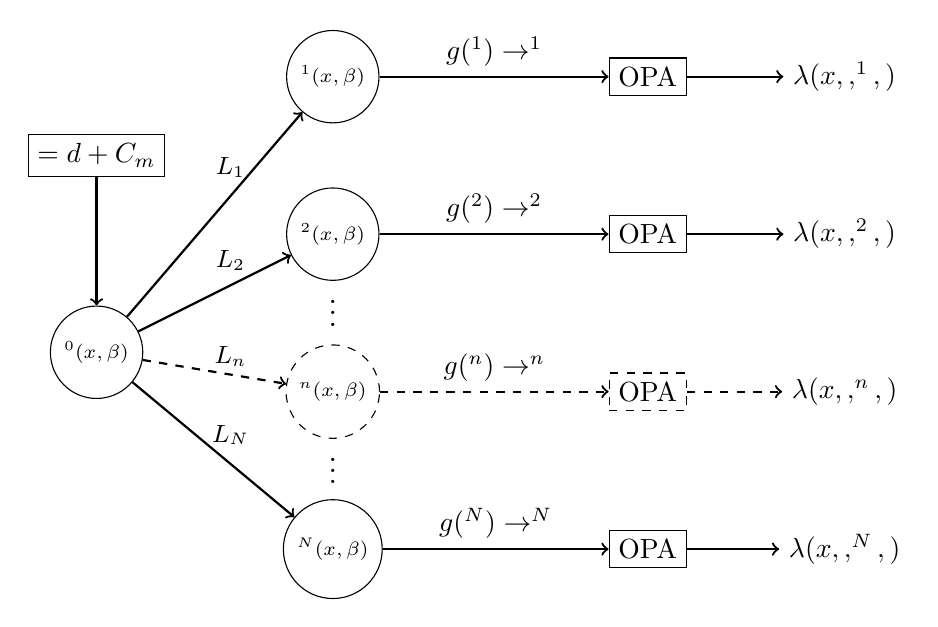
\begin{tikzpicture}

\draw (.5,3) node(INPUT)[rectangle,draw]{ $\rd=d + C_m \ri$};

\draw (.5,.5) node(ROOT)[circle,draw]{\scriptsize $\ry^0(\alert{x},\alert{\beta})$ };
\draw (3.5,4) node(ONE)[circle,draw]{ \scriptsize $\ry^1(\alert{x},\alert{\beta})$ };
\draw (3.5,2) node(TWO)[circle,draw]{ \scriptsize $\ry^2(\alert{x},\alert{\beta})$ };
\draw (3.5,1.1) node(DOTONE){ \large $\vdots$ };
\draw (3.5,0) node(N)[circle,dashed,draw]{ \scriptsize $\ry^n(\alert{x},\alert{\beta})$ };
\draw (3.5,-.9) node(DOTTWO){ \large $\vdots$ };
\draw (3.5,-2) node(S)[circle,draw]{ \scriptsize $\ry^N(\alert{x},\alert{\beta})$ };

\draw (2.2,2.85) node(OMG1){ \small $L_1$ };
\draw (2.2,1.67) node(OMG2){ \small $L_2$ };
\draw (2.2,.45) node(OMG){ \small $L_n$ };
\draw (2.2,-.55) node(OMGS){ \small $L_N$ };

\draw[thick, ->] (INPUT) -- (ROOT) ;
\draw[thick, ->] (ROOT) -- (ONE) ;
\draw[thick,->] (ROOT) -- (TWO);
\draw[thick,dashed, ->] (ROOT) -- (N);
\draw[thick,->] (ROOT) -- (S);

\draw (7.5,4) node(OPAONE)[rectangle,draw]{ OPA  };
\draw (7.5,2) node(OPATWO)[rectangle,draw]{ OPA  };
\draw (7.5,0) node(OPAN)[rectangle,dashed,draw]{ OPA  };
\draw (7.5,-2) node(OPAS)[rectangle,draw]{ OPA };

\draw[thick, ->] (ONE) -- (OPAONE) node [midway,above] { $g(\ry^1) \rightarrow \rxi^1$ };
\draw[thick,->] (TWO) -- (OPATWO) node [midway,above] { $g(\ry^2) \rightarrow \rxi^2$ };
\draw[thick,dashed, ->] (N) -- (OPAN) node [midway,above] { $g(\ry^n) \rightarrow \rxi^n$ };
\draw[thick,->] (S) -- (OPAS) node [midway,above] { $g(\ry^N) \rightarrow \rxi^N$ };


\draw (10,4) node(ONEFIN)[rectangle]{ $\lambda (x,\rd,\rxi^1,\romega )$  };
\draw (10,2) node(TWOFIN)[rectangle]{ $\lambda ( x,\rd,\rxi^2,\romega )$ };
\draw (10,0) node(NFIN)[rectangle,dashed]{ $\lambda ( x,\rd,\rxi^n,\romega )$ };
\draw (10,-2) node(SFIN)[rectangle]{ $\lambda ( x,\rd,\rxi^N,\romega)$ };

\draw[thick, ->] (OPAONE) -- (ONEFIN) ;
\draw[thick,->] (OPATWO) -- (TWOFIN);
\draw[thick,dashed, ->] (OPAN) -- (NFIN);
\draw[thick,->] (OPAS) -- (SFIN);


%\draw[thick,dashed] (TWO) -- (N);
%\draw[thick,dashed] (N) -- (S);

\end{tikzpicture}
\caption{JCC $N-1$ Risk Model to seed random initial contingencies for OPA}\label{high_level_sample}
\end{figure}




The OPA cascade in this sense is used as a surrogate function to represent rare event risk for a given topology.  The following are the inputs to OPA model that has multiple stages and is solved via multiple LP programs.  The first is the controllable generation $x$, which also indirectly controls the line failure distributions through the intermediate variable $\ry$.  The second input for the OPA model is $\rd$, which is also used directly in our JCC model.  The third input is the initial contingencies $\rxi$, which depends on $\ry$, and thus on $x$ and $\rd$.  Finally, we have $\romega$, which governs the evolution of the cascade process. The load shed for a particular realization of an OPA run is represented by $\lambda$ and is the difference between the nominal load and the load at the last stage of the cascade in the OPA simulation.
\begin{equation}
\lambda ( x, \rd, \rxi, \romega )
\end{equation}
We are using the expected load shed as a weighting factor to measure the impact of a particular line failure on the OPA cascading process.  For each contingency $n$, we have a different set of random initial contingencies due to the choice of generation $x$, slack distribution $\beta$ and the resulting random flows $\ry^n$ for each contingency.  The expected load shed for contingency $n$ is
\begin{equation*}
f_n = \E{\bD, \Xi,\Omega}{ \lambda\left(x,\rd,\rxi^n,\romega\right) }.
\end{equation*}



\begin{algorithm}
\caption[Contingency sampling algorithm for OPA]{Contingency Sampling Algorithm for OPA.  Given a dispatch $(x, \beta)$, random demand $\rd=d_0 + C_m \ri$, sample $\rxi^n$ for $T$ trials for each $N-1$ Contingency \Cref{high_level_sample}}\label{opa_sample_alg}
\begin{algorithmic}
\Procedure{SAMPLE}{$x,\beta, \ri, T$}
\For{$\forall t = 1,2,...,T^\bD$}
\State Sample $a=(a_1,a_2,...,a_N)^T$ from independent standard normal distributions.
\State $H H^T = \Sigma^m$ using Cholesky decomposition
\State $\delta^m = H * a$, which has the desired distribution due to affine transformation
\State $\Delta = \sum_m \delta_m$
\State $x=C_g(x_0 + \beta \Delta)  -(d_0 + C_m \delta^m)$ using \Cref{rand_inj} 
\State $y=y_0 + A C_G \beta \Delta - A C_m \delta^m$ using \Cref{rand_flow}
\For{$ \forall n \in \cE \mbox{s.t.} A_{nn}^B \neq 1$}
\State $L_{e n} = A^B_{en}(1-A^B_{nn})^{-1}$ using \Cref{line_outage}
\State $y_e^n = y_e + L_{e n} y_n$  using \Cref{n1cont}
\State $z_e^n = g_e (y_e^n)$

\State $\mathbb{O}^n \gets \emptyset$
\For{$\forall t = 1,2,...,T^\Xi$}

\For{$\forall e \in \cE $}
\State $\xi_e = 
\left\{ 
\begin{array}{lr}
  1 & \mbox{w/ prob. } z_e^n \\
  0 & \mbox{o/w }
\end{array}
\right. $ 
\EndFor
\State $\mathbb{O}^n \gets \xi$
\EndFor
\EndFor
\EndFor
\State The set $\mathbb{O}^n$ of initial contingencies for each $N-1$ contingency, representing distribution $\rxi^n$
\EndProcedure
\end{algorithmic}
\end{algorithm}





\subsection{OPA Weighting for JCC}


While it is important that no lines fail, it may be overly restrictive while not actually reducing the risk of large load shedding events, which is a main concern from a system reliability perspective. It would certainly be more beneficial to keep the large high voltage lines in operation that are critical to system stability versus a few small distribution feeders, which may cause some small load shedding but would keep the bad events contained.  To highlight the downside of chance constrained programming of not capturing the impact of the events,  a scatter plot in  \Cref{jcc_and_opa} of the system risk measure of the JCC model and the expected load shed of the OPA model seeded by the random initial contingencies from \Cref{opa_sample_alg}, we see there is not a good correlation.  We want to develop a system constraint that is correlated with the expected load shed from the cascading process.

\begin{figure}
\centering
\begin{tikzpicture}[scale=.9]
\begin{axis}[title=Risk Measure vs Load Shed, xlabel=Load Shed, ylabel={$P \left[ \mbox{At least one line fails} \right]$},legend pos=outer north east]
%,ymax=.04%,xmin=\xmmm,xmax=1,
%	  extra x ticks={.8,.9,.98},
%	  extra x tick style={grid=major},
%	  extra x tick labels={}]


  \addplot+[blue,opacity=.85,only marks, mark size=.35] table[x=LS,y=r] {\mypathojdata/jccS1.out};
  \addlegendentryexpanded{JCC}
  \addplot+[blue,opacity=.85,only marks, mark size=.35] table[x=LS,y=r] {\mypathojdata/jccS2.out};
  \addplot+[blue,opacity=.85,only marks, mark size=.35] table[x=LS,y=r] {\mypathojdata/jccS3.out};
  \addplot+[blue,opacity=.85,only marks, mark size=.35] table[x=LS,y=r] {\mypathojdata/jccS4.out};
  \addplot+[blue,opacity=.85,only marks, mark size=.35] table[x=LS,y=r] {\mypathojdata/jccS5.out};


\end{axis}
\end{tikzpicture}
\caption{Line failure risk and OPA not correlated}\label{jcc_and_opa}
\end{figure}


For each line $e$, we construct a risk-weighting $\eta_e$ such that the expected value of the load shed distribution after losing that line is equal to $\eta_e$.  
\begin{align} \label{jcc_ow_weights}
\sum_e \eta_e \E{\bD}{g(\ry_e^n(\alert{x},\alert{\beta}))} &\approx \E{\bD, \Xi^n, \Omega}{\lambda ( \alert{x},\rd,\rxi^n,\romega) } \\
\eta^T z^n &\approx f_n
\end{align}


\bc{\begin{figure}
\centering
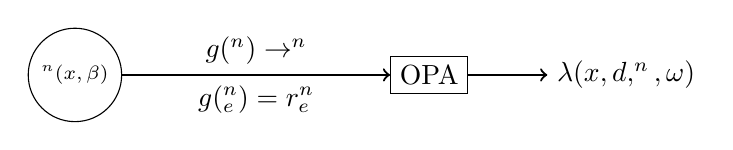
\begin{tikzpicture}
\draw (3.5,4) node(ONE)[circle,draw]{ \scriptsize $\ry^n(\alert{x},\alert{\beta})$ };

\draw (8,4) node(OPAONE)[rectangle,draw]{ OPA  };

\draw[thick, ->] (ONE) -- (OPAONE) node [midway,above] {$g(\ry^n) \rightarrow \rxi^n$ } node[midway,below]{$\E{\bD}{g(\ry_e^n)} = r_e^n$};

\draw (10.5,4) node(ONEFIN)[rectangle]{ $\lambda (\alert{x},d,\rxi^n,\omega )$  };

\draw[thick, ->] (OPAONE) -- (ONEFIN) ;

%\draw<2->[thick,dashed,red] (4.45,3.8) -- (7.2,3.8) -- (7.2,4.8) -- (4.45,4.8) -- (4.45,3.8);
\end{tikzpicture}
\caption{Random initial contingencies and expected failure probabilities}
\end{figure}
}

There are many ways to find a weighting scheme to represent the impact from losing particular lines.  Here is one example that attempts to capture the impact of losing a line with respect to the effect on the expected load shed of the resulting OPA simulations.  For each contingency, a vector of risk levels, $z^n$, were recorded, which represent the expected probability of line $e$ failing under contingency $n$ (  for contingency $n$, the probability of line $n$ failing is  $z^n_n=1$).  After performing the OPA simulations, we record the expected load shed $f_n(x)$ for that set of initial contingencies $\rxi^n$.  We formulate the following linear system \Cref{solve_opa_weight} and solve for $\eta$.
\begin{equation*}\label{solve_opa_weight}
\begin{bmatrix}  \alert{z^1_1} & \cdots & \alert{z^1_{N_l}} \\ \vdots & \vdots & \vdots \\ \alert{z^{N_l}_1} & \cdots & \alert{z^{N_l}_{N_l}} \end{bmatrix}
\begin{bmatrix} \alert{\eta_1}  \\ \vdots  \\ \alert{\eta_{N_l}}  \end{bmatrix} 
=
\begin{bmatrix} \alert{f_1}  \\ \vdots  \\ \alert{f_{N_l}}  \end{bmatrix} 
\end{equation*}

After applying these new linear weights $\eta$ to the line risks $z$, we find that our new system constraint $\sum_e \eta_e z_e$ is now well correlated with the resulting expected value of load shed of the cascading process as shown in \Cref{jcc_ow_correlated}.
In order to solve problems using this weighting scheme, it is nearly identical to JCC $N-1$ model\Cref{jcc_n1_program}, except with the system risk constraint \Cref{n1linerisk} representing probability of one or more line failures with the new risk constraint representing the expected value of load shed \Cref{jcc_ow_weights}.

\begin{subequations}
\label{jcc_n1_ow_program}
\begin{alignat}{3}
\textbf{JCC $N-1$ OW:= }\min_{\left(x,\beta,;\theta,y,\pi,s,z\right)} & \displaystyle\sum_j \left[  c_2 \left(x_j^2 + \beta_j^2 \sD \right) + c_1 x_j + c_0 \right] &&  \label{ow_obj}  \\
&\Cref{jcc_cons,jcc_kcl,jcc_limit,jcc_gen1,jcc_gen2,jcc_slack,jcc_pi,jcc_var,jcc_lr,jcc_risk}   && \nonumber\\
&\Cref{n1meanup,n1meandown,n1stddev,n1linerisk}   && \nonumber\\
&\sum_e \eta_e z_{en} \leq \zeta_n && \forall n \in \cE
\end{alignat}
\end{subequations}

\begin{figure}
\centering
\begin{tikzpicture}[scale=1]
\begin{axis}[title=Risk Measure vs Load Shed, xlabel=Load Shed, ylabel=JCC-OW Risk Measure,legend pos=outer north east]
%,ymax=.04%,xmin=\xmmm,xmax=1,
%	  extra x ticks={.8,.9,.98},
%	  extra x tick style={grid=major},
%	  extra x tick labels={}]


  \addplot+[blue,opacity=.85,only marks, mark size=.35] table[x=LS,y=rl] {\mypathojdata/jccS1.out};
  \addlegendentryexpanded{JCC}
  \addplot+[blue,opacity=.85,only marks, mark size=.35] table[x=LS,y=rl] {\mypathojdata/jccS2.out};

  \addplot+[blue,opacity=.85,only marks, mark size=.35] table[x=LS,y=rl] {\mypathojdata/jccS3.out};

  \addplot+[blue,opacity=.85,only marks, mark size=.35] table[x=LS,y=rl] {\mypathojdata/jccS4.out};

  \addplot+[blue,opacity=.85,only marks, mark size=.35] table[x=LS,y=rl] {\mypathojdata/jccS5.out};


\end{axis}
\end{tikzpicture}
\caption{JCC $N-1$ OW correlated with OPA} \label{jcc_ow_correlated}
\end{figure}





\subsection{Cutting Plane Algorithm for JCC $N-1$ with OPA Weighting}
Now, we describe the algorithm used to solve  JCC $N-1$ \Cref{jcc_n1_program} and the new JCC OW \Cref{jcc_n1_ow_program}.  The algorithm for JCC OW is shown explicitly in \Cref{jcc_ow_alg} and the JCC $N-1$ is nearly identical except for the difference in system risk constraints.
\begin{algorithm}
\caption[Cutting plane algorithm for solving JCC $N-1$ with OPA weighting]{This cutting plane algorithm solves JCC \Cref{jcc_program} with $N-1$ contingencies \Cref{jcc_n1_program} using the OPA weighting scheme \Cref{jcc_ow_weights} via linear programs and cutting planes}\label{jcc_ow_alg}
\begin{algorithmic}
\Procedure{JCC $N-1$ OW}{d,$\Sigma^m$,$\zeta$,$\zeta_n$,L,p}
\State $L^n \gets \emptyset$  (Set of Lines with potential risk for contingency $n$)
\State $S \gets \emptyset$  (Set of Cuts)
\State $r \gets 0$ (Risk)
\BState \emph{solve}:
\State $(\hat{x},\hat{\beta},\hat{y}) \gets $Solve DC Power Flow, \Cref{jcc_obj,jcc_cons,jcc_kcl,jcc_slack,jcc_limit,jcc_gen1,jcc_gen2}, with cuts $S$, risk $r\leq\epsilon$
\If {Infeasible} \Return Problem Infeasible 
\EndIf
\State $N_f \gets 0$
\For{$\forall n$}
\State Calculate branch flows $\hat{y^n}$ for contingency $n$ using \Cref{n1cont}
\State Calculate $\hat{s^n},\hat{z^n},\hat{r^n}$ using $(\hat{x},\hat{\beta},\hat{y})$ and \Cref{n1var}
\If {$\hat{r} \geq \epsilon + tol$} $N_f = N_f + 1$
\EndIf

\For{$\forall e$}
\If {$\hat{z^n_e} \geq tol$}
    \If {$e \notin L^n$}
            \State $L^n \gets \left\{L^n,e\right\}$
            \State Initialize $s^n_e,z^n_e$
            \State $r^n \gets r^n + z^n_e$
    \EndIf            
    \State $S \gets$ line risk cuts \Cref{line_risk_cuts} for $z^n_e,y^n_e,s^n_e$ dependent on $\hat{z}^n_e,\hat{y}^n_e,\hat{s}^n_e$
    \State $S \gets$ branch variance cuts \Cref{sd-cuts} for $s^n_e,\beta_e$ dependent on $\hat{s}^n_e,\hat{\beta}_e$
\EndIf
\EndFor
\EndFor
\If{ $N_t = 1$ } \Return Optimal $(\hat{x},\hat{\beta},\hat{y})$
\Else
\State \textbf{goto} \emph{solve}
\EndIf
\EndProcedure
\end{algorithmic}
\end{algorithm}



\section{Computational Experiments}
This computational section shows an example of using the OPA weighting on top of the JCC model enchanced with $N-1$ contingency considerations. We began by  running JCC $N-1$  and used it to initiate the $N-1$ OPA sampling process and ran OPA on each initial contingency.  We created an OPA weighting vector as described in \Cref{solve_opa_weight}.  Then we solved JCC OW \Cref{jcc_n1_ow_program} using cutting plane algorithm \Cref{jcc_ow_alg}.  Finally, we ran the $N-1$ OPA process again with the two models to determine load shed distribution associated with the two dispatch points.   The goal for the JCC OW model is to modify the distribution of load shed and reduce the risk of rare event failures that are large.  

To highlight the differences of the JCC OW model, this trial gave a higher budget to the JCC OW model and constrained the new system risk measure so that the cost of dispatch was 4\% higher than the standard JCC model.  In return, it was able to reduce the expected value of load shed by 4.7\%, and reduce the 99 percentile of load shed by 28.5\%.  Some statistical measures of the load shed distribution are shown in \Cref{rare_event_risk_metrics} and plotted in \Cref{load_shed_dist_ow}.  In the plot \Cref{load_shed_dist_ow}, we have the load shed distribution shown on the left where each picture is zoomed in to see the tail of the distribution.  On the right side, we have a log plot of the number of trials that are in each bin.  In \Cref{rare_event_risk_metrics}, we have the cost of the dispatch point as well as statistics on the resulting load shed distribution.  We have tabulated the mean, the number of trials with no load shed, the 95th, 99th, and 99.8th percentiles.  Additionally, we have the maximum over all trials as well as the conditional value at risk of the 95th percentile.

\begin{figure}
\centering
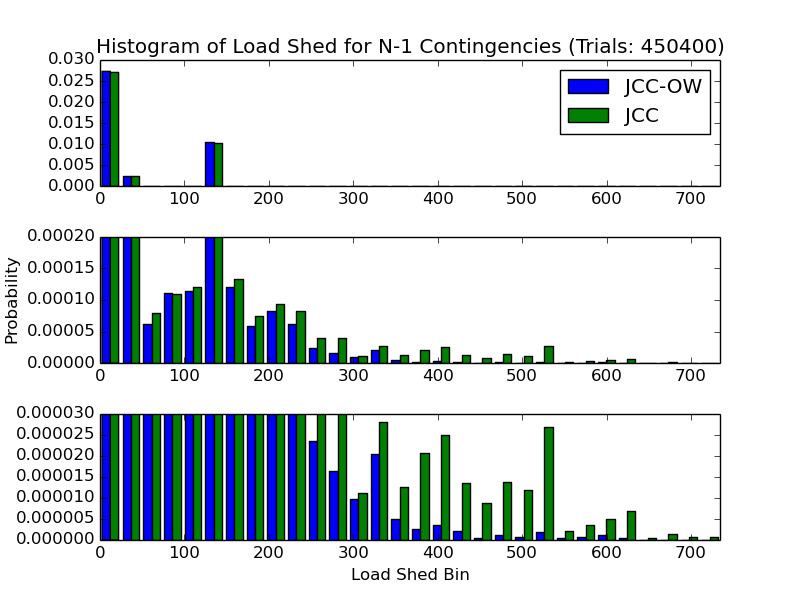
\includegraphics[scale=.4]{\mypathoj/histogram-newdes3}
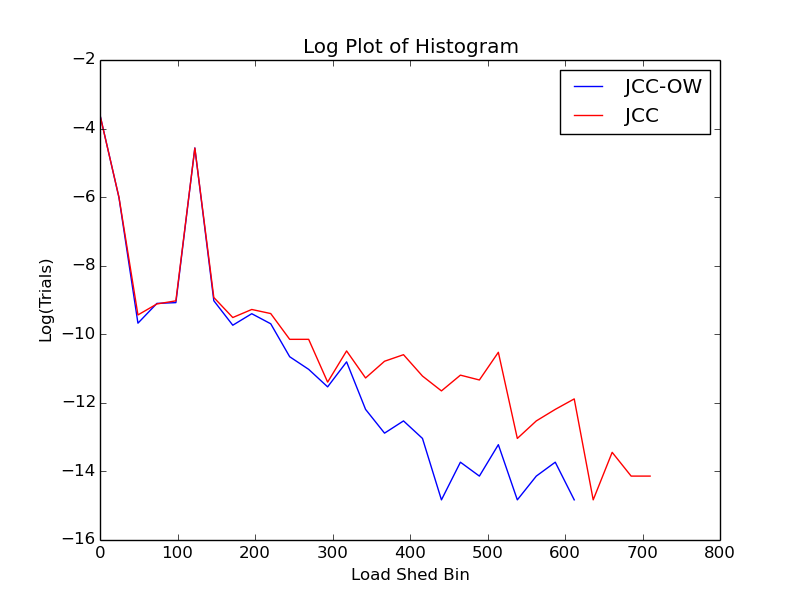
\includegraphics[scale=.4]{\mypathoj/logplot-newdes3}
\caption{Load shed distribution}
\label{load_shed_dist_ow}
\end{figure}


\begin{table}
\centering
Trials \textbf{450400}

\begin{tabular}{|c |  c c | c|}
\hline
Stat & JCC & JCC-OW & diff (\%) \\
\hline
cost&1.78e6 & 1.85e6 & \alert{-3.9} \\
mean&44.0&41.9 & 4.8   \\
No Load Shed&199444 & 201984 & 1.3 \\
P95& 138.81& 138.81  &  0         \\
P99& 205.77& 147.12456 &  28.5        \\
P99.8& 441.21& 251.76   &  43      \\
max& 734.29& 612.9      &  16.5            \\
CVaR95 & 182.5 & 155.6 & 14.7 \\
\hline
\end{tabular}
\caption{Rare event risk metrics}\label{rare_event_risk_metrics}
\end{table}


\section{Conclusion}
In this Chapter, we extended the JCC model to include the security constrained, $N-1$ contingencies.  Additionally, we take into account the approximate impact of losing subsets of lines on the resulting OPA cascading process.  We use the OPA cascading process as an empirical model to represent how stressed the grid is with respect to rare event failures.  The OPA process gives us a distribution of load sheds and we use this distribution to develop risk-weighting factors for the lines.  The JCC OW model, which incorporates this linear weighting scheme, was able to change the distribution (for an increased cost) of the resulting load shed by reducing the mean and, even more so, reducing the tail events with large load shed.
